\documentclass{article} 
\usepackage[utf8]{inputenc}
\usepackage[T2A]{fontenc}
\usepackage[russian, english]{babel}
\usepackage{graphicx}	
\usepackage{amsmath, amssymb}
\usepackage{titlesec}
\newcommand\tab[1][1cm]{\hspace*{#1}}
\usepackage[14pt]{extsizes}
\usepackage{setspace,amsmath}
\usepackage[left=20mm, top=15mm, right=15mm, bottom=15mm, nohead, footskip=10mm]{geometry} 
\usepackage{mathtext}
\usepackage[dvipsnames]{xcolor}
\usepackage{ragged2e}
\sloppy
\usepackage{caption}
\usepackage{hyperref}

\hypersetup{
    colorlinks=true,
    linkcolor=black,
    urlcolor=blue
}

\graphicspath{ {img/} }
%--------------------------------------------------------------------
\begin{document}                                                         
\newpage
\thispagestyle{empty}

\begin{center}
Федеральное государственное образовательное бюджетное учреждение\\ высшего профессионального образования\\ 
\textbf{«Финансовый университет при Правительстве Российской Федерации»}\\
\end{center}
	
\vspace{2em}
	
\begin{center}
\textbf{Департамент анализа данных, принятия решения и финансовых технологий}\\ 
\end{center}
	
\vspace{2em}
	
\begin{center}
\textbf{Курсовая работа\\
\vspace{3mm}}
по дисциплине \textbf{"Технологии анализа данных и машинное обучение"} на тему: \\ \vspace{2em} \textbf{"Классификация текстов методами машинного обучения"}\\
\vspace{3mm}
Вид исследуемых данных: Корпус новостей с сайта Lenta.Ru\\
\end{center}
	
\vspace{6em}
		
\begin{flushright}
Выполнила:\\
студентка группы ПМ17-1\\
Баданина Н. Д.\\
Научный руководитель:\\
доктор техн. наук, профессор\\
Судаков Владимир Анатольевич
\end{flushright}
	
\vspace{\fill}
	
\begin{center}
Москва 2020
\end{center}

%--------------------------------------------------------------------
\newpage
	
\renewcommand*\contentsname{Содержание}
\makeatletter
\renewcommand{\l@section}{\@dottedtocline{1}{0em}{2em}}
\renewcommand{\l@subsection}{\@dottedtocline{1}{0em}{2.6em}}
\renewcommand{\l@subsubsection}{\@dottedtocline{1}{0em}{3.2em}}

\makeatother
\setcounter{page}{2}

\begin{center}
	\tableofcontents
\end{center}
%--------------------------------------------------------------------
\newpage
\addcontentsline{toc}{section}{Введение}
\section*{Введение}
\tabНа сегодняшний день технологии развиваются с экспоненциальной скоростью. Это значит, что за следующий десяток лет появится больше инновационных продуктов, чем за предыдущий десяток. За короткий период времени в научном мире развилась целая новая область знаний, которая требует изучения — это Искусственный Интеллект (ИИ, artificial intelligence, AI). В AI, как подраздел, можно включить машинное обучение (machine learning, ML), алгоритмы машинного обучения. В свою очередь алгоритмы ML можно условно разделить на четыре направления. Первое направление — классическое обучение. В него входят такие методы, как классификация, регрессия, кластеризация, уменьшение размерности и другие. Часть перечисленных методов реализованы в данной работе. Оставшиеся направления включают в себя нейронные сети и глубокое обучение, обучение с подкреплением, ансамблевые методы.\\
\tabПик развития машинного обучения начался ориентировочно в 2015 году, когда бизнесы начали активно цифровизироваться, уходить в онлайн, для чего им понадобилось внедрение большого числа современных цифровых технологий, в том числе методов машинного обучения. Также, развитие алгоритмов обусловлено борьбой за клиентов, которым важна и безопасность продукта, и доступность, и персонализация. Это подтолкнуло компании к вложению средств в изучение области AI.\\
\tabВ данной работе речь пойдет об алгоритмах классификации и обработки текста на естественном языке. Эти разработки активно используются при создании голосовых помощников, чат-ботов, умных устройства для дома. Технологии, основанные на распознавании естественных языков создают новый интерфейс для взаимодействия с пользователем. К примеру, пользователю достаточно устно озвучить запрос, не вводя ничего привычным способом. В речевом анализе аудиоданные преобразуются в текст, к которому можно применить алгоритмы Natural Language Processing (NPL) — методы обработки текстов на естественном языке.\\
\tabТакже примером внедрения анализа естественного языка может служить поддержка "тегов рекомендаций", реализованная у Netflix, YouTube. Тег — это метоинформация о фрагменте контента, важная для поиска и рекомендации. Теги определяют свойства описываемого ими объекта и могут быть использованы для группировки схожих элементов и предложения описательных названий для таких групп. Широкое использование теги получили в электронных новостных изданиях, к примеру Я.Дзен, Lenta.ru, Тинькофф Журнал. Для выполнения практической части курсовой работы мною были взяты размеченные данные с сайта Lenta.ru. Данные содержат текст новости, заголовок, тег.\\
%--------------------------------------------------------------------
\subsection{Сложности при обработке текстов на естественном языке}
\tabОсновной сложностью при обработке текстов на естественном языке программными средствами является понимание алгоритмом контекста, в рамках которого идет обработка отдельного слова. Зачастую в тексте используются слова в переносном значении или в значении, которое установили собеседники между собой по договоренности. Особенно часто такое происходит в профессиональной литературе. При существовании множества смыслов язык становится избыточен. Избыточность является серьезной проблемой при построении алгоритмов NLP, так как разработчик такой системы не сможет и не будет указывать буквальный смысл каждого ассоциативного слова.  \\
\tabСледующая проблема связана со свойством слов менять свое значение с течением времени. Единицей анализа текста является лексема — слово как абстрактная единица морфологического анализа. Лексема "батарея" изменила свой смысл с течением времени. Так, в текстах 20 века и ранее можно увидеть это слово для обозначения артиллерийского подразделения из нескольких орудий. В современных публикациях лексема используется для обозначения хранилища, преобразующего химическую энергию в электронную.\\
\tabСпециалисты по обработке и анализу текстов также сталкиваются с проблемой высокой и низкой энтропии. Это означает, что в системе в большей или меньшей мере существует мера неопределенности, в частности непредсказуемость появления какого-либо символа алфавита. Рассмотрим задачу восстановления пропущенного слова в предложении. Фразеологизм "мастер на все ..." имеет низкую энтропию, то есть существует мало слов, которые подойдут для завершения предложения, тогда как "встретимся около ..." предполагает множество вариантов. Человек способен использовать не только контекст, но и предыдущие знания, чтобы ответить. Однако, компьютерные модели не обязательно обладают этой информацией.\\
%--------------------------------------------------------------------
\subsection{Перспективы развития технологии}
\tabРазвитие технологии классификации текстов началось с введения спам-фильтров для почты. В 20 веке электронные письма были не распространены, поэтому защитить почту от мошенников можно было точечной блокировкой адресов. С распространением технологии уже трудно представить ручную регулировку. Это подтолкнуло разработчиков к созданию первых алгоритмов классификации текстов. Развитие технологии классификации мошеннических писем остается актуальной и на сегодняшний день в связи с увеличением сервисов для коммуникации: Telegram, WhatsApp, mail и так далее. В перспективе с помощью этих же моделей можно классифицировать незаконные банковские транзакции, транзакции с участием криптовалют.\\
\tabТехнологические гиганты также ищут способ оптимизации процессов. Рекомендательные системы позволяют им получать дополнительную прибыль и основывать бизнес стратегию на AI системах. В свою очередь, при построении рекомендаций фильмов, книг, новостей необходимо учитывать текстовые данные, указанные у объекта: заголовок, отзыв, рецензия, тег, категория. Правильно настроенная модель классификации текстов в перспективе улучшит работу рекомендательных движков, которые в свою очередь генерируют прибыль сервисов.\\
\tabПриложения, основанные на использовании естественного языка только начинают распространяться, но в будущем могут взять на себя задачи, которые сейчас решаются стандартными формами и  интерфейсами.\\
%--------------------------------------------------------------------
\newpage
\section{Теоретическая часть} 
%--------------------------------------------------------------------
\subsection{Задачи классификации текстов}
Основные задачи NLP: \\
\tab1) Классификация текстов. Модели направлены на определение текста к тому или иному классу исходя из его признаков и особенностей.\\
\tab\tab— фильтрация спама. Целевой переменной выступает булева переменная, принимающая значение 1 или 0 в случае наличия или отсутствия в письме спама соответственно. \\
\tab\tab— анализ тональности. Применяется для классификации отзывов, сообщений, твитов по положительному, отрицательному или нейтральному отношению автора.\\
\tab\tab— определение интента, то есть намерения пользователя. К примеру, при вводе поискового запроса система "подсказывает" возможные продолжения.\\
\tab\tab— деление текстов по теме/жанру/тегу. Эта задача реализована в практической части данной работы.\\
\tab2) Кластеризация текстов. Разбиение коллекции документов на кластеры, то есть на подмножества близких по темам документов.\\
\tab\tab— агрегация новостей. Агрегатор осуществляет сбор и систематизацию новостей так, что интернет-пользователь может искать информацию в создаваемом информационном массиве по ключевым словам, при этом исключаются неновостные ресурсы, которые также могут содержать ключевые слова.\\
\tab\tab— рекомендации. Кластеризация документов, построение рекомендаций.\\
\tab3) Извлечение информации.\\
\tab\tab— именованные сущности (Named-entity recognition, NER). Задача NER — выделить спаны сущностей в тексте, где спан — непрерывный фрагмент текста. Заранее определяется некоторый фиксированный набор — например, люди, места, организации, время и так далее. Из текста необходимо выделить слова, которые принадлежат одному из наборов.\\
\tab\tab— выделение атрибутов объектов и семантических отношений между ними.\\
\tab4) Машинный перевод. Является одной из самых ранних разработок в сфере NLP. Первые модели использовали стратегию пословного перевода, но быстро стало понятно, что необходимо учитывать и другие лингвистические модели. Несмотря на долгое время существования, качество машинного перевода все ещё далеко до отличного. Прорыв в этой области основан на возникновении нейронный сетей, на основе которых работают интернет переводчики от Google, Яндекс.\\
\tab5) Вопросно-ответные системы. Одно из самых частых применений — чат-боты, которые используются в совершенно разных отраслях, включая даже банки.\\
\tab6) Генерация текстов. Технологии машинного обучения позволяют создавать оригинальные тексты, указав, к примеру, начальное слово.\\
\tab7) Распознавание речи. Активно применяется при создании голосовых помощников.\\
\tab8) Проверка правописания.\\
\tab9) Реферирование текста (Summarization), то есть сокращение объема текста и получение краткого изложения содержания. Также саммаризацию можно выполнять по нескольким близким документам, к примеру по новостям. Близкой задачей является аннотирование текста, то есть выделение ключевых тем.
%--------------------------------------------------------------------
\subsection{Формализация процесса обработки текста} 
%--------------------------------------------------------------------
\subsubsection{Разметка текстовых данных} 
\tabРазмеченные данные, то есть такие, у которых известна целевая переменная, например категория, можно анализировать с помощью методов ML с учителем. "Учителем" выступают сами разметки, так как однозначно понятно какой ответ разработчикам хотелось бы получить от алгоритма. Данные имеют метки, то есть понятно, к каким категориям принадлежат записи. Обычно быстрее, проще и дешевле найти и разметить достаточно данных, на которых будет обучаться модель — вместо того, чтобы пытаться оптимизировать сложный метод обучения без учителя, когда разметка отсутствует. 
%--------------------------------------------------------------------
\subsubsection{Токенизация} 
\tabТокенизацией называют разбивку текстов на более мелкие части — токены. Чаще всего стоит задача разбивки текста на слова, однако, к токенам относятся как слова, так и знаки пунктуации. Возможна разбивка на запятые, цифры, это зависит от задачи. Зачастую необходимо представить текст в виде массива значимых слов. В этом случае после токенизации необходимо удалить знаки пунктуации и незначимые слова, например предлоги.
%--------------------------------------------------------------------
\subsubsection{Исправление опечаток}
\tabВ редких случаях в процесс обработки текста включают исправление опечаток. Дело в том, что это очень трудоемкий и кропотливый процесс, которые скорей всего не увеличит точность работы модели. Однако, в отдельно взятых случаях он необходим.
%--------------------------------------------------------------------
\subsubsection{Сегментация предложений}
\tabВ зависимости от задач, может потребоваться токенизация не по словам, а по предложениям. К примеру, для решения задачи саммаризации. В таком случае предстоит разделить текст на предложения. Сложность заключается в определении конца и начала, так как не всегда предложение заканчивается точкой, может стоять восклицательный, вопросительный знак. Также не всегда точка значит конец, знак используется для сокращений, обозначений дат. Заглавная буква также может встречаться как в начале, так и в именах, названиях и не является неоспоримым признаком начала предложения.
%--------------------------------------------------------------------
\subsubsection{Лемматизация. Cтемминг}
\tabЛемматизация — приведение слов к начальной форме. Это необходимо, так как при представлении текста в векторном пространстве, слова с разными формами, но одинаковым значением будут считаться как разные признаки. Считается, что для каждого токена существует его нормальная форма или лемма. От этой начальной формы создаются все остальные формы слова путем флексии, то есть изменений этой начальной формы. Рассмотрим пример на слове "сделали": сделал — основа, частица -и — флексия.\\
\tabВведем новый термин — словоформа. Под словоформой будем понимать группу, состоящую из токена, связанной с ним начальной формы и множества грамматических параметров. Тогда, исходя из данного определения, можно сказать, что задачей лемматизации является нахождение в словаре словоформы по её токену.\\
\tabПри анализе текстовых данных можно считать количество словоупотреблений токенов, однако, аналогично, лучше рассчитывать сколько раз встретилась каждая из лексем, чтобы избежать дублирования слов разной формы. Для этого необходимо предварительно провести лемматизацию. В итоге выполнения преобразований получится вектор. Вектор может быть построен как для лемм, так и для словоформ или токенов, в зависимости от того, какая задача стоит перед разработчиками.\\
\tabВекторное представление позволяет перейти от текста к его описанию в некотором пространстве. Каждая лемма задаёт собственное направление в неком многомерном пространстве, размерность которого будет равна количеству лемм в тексте. В таком случае, текст можно представить как точку или вектор в этом многомерном пространстве. Переход к многомерному пространству позволяет измерять расстояния между текстами, то есть степень, в которой они похожи или не похожи друг на друга. Если в двух текстах употребляются одни и те же слова, то эти тексты посвящены одной или сходной теме.\\
\tabВ зависимости от постановки задачи, морфологический анализатор может возвращать разную информацию. Если необходимо рассчитать вектор частотности употребления слов в тексте, то необходимо использовать только лемму или лемму с указанием части речи. Для языков с невысокой флективностью применяется стемминг, то есть определение основы слова путём отбрасывания окончаний из известного набора. Отличие стемминга от лемматизации можно продемонстрировать на примере слова выходцы: процесс лемматизации определит лемму выходец, в то время как стемминг вернёт псевдооснову выход. При анализе корпусов на русском языке предпочтительнее использовать лемматизация в виду разнообразия основ и превдооснов языка.
%--------------------------------------------------------------------
\subsubsection{Извлечение ключевых слов}
\tabКлючевые слова — это лексические группы, отражающие содержание документа. Проблематичным является автоматическое извлечение многокомпонентных ключевых слов. При всех методиках, алгоритм извлечения ключевых слов универсален и включает этапы:\\
\tabа) формирования множества «кандидатов» в ключевые слова\\
\tabб) фильтрации этого множества для получения результирующего списка ключевых слов.\\
\tabДостаточно часто до извлечения ключевых слов из текста удаляются стоп-слова. Стоп-слова – это слова, которые не несут никакой смысловой нагрузки (артикли, предлоги, союзы, частицы, местоимения, вводные слова, междометия и так далее)
%--------------------------------------------------------------------
\subsubsection{Модель представления текста}
\tabМодель представления текста в векторном пространстве. Label Encoding (LE) — простой подход, основанный на переводе каждого значения в цифру. Категориальные значения сортируются и им присваиваются упорядоченные порядковые номера. Используется для кодировки меток в датасете.\\
\begin{center}
\begin{tabular}{||c | c||} 
\hline
 Animal Category & LE \\ [0.5ex] 
 \hline\hline
 Dogs & 0 \\ 
 \hline
 Cats & 1 \\
 \hline
 Birds & 2\\ [1ex] 
 \hline
\end{tabular}
\end{center}
\tab LE прост в применении, однако его минусом является то, что другие алгоритмы ML могут принять численные категории как иерархию, увидеть порядок в них. Эта проблема исправляется в алгоритме One-Hot Encoding (OHE). Каждый признак конвертируется в новую колонку. Признакам присваивается значение 1 или 0 в зависимости от соответствия новой колонки и первоначального признака.\\
\begin{center}
\begin{tabular}{||c | c | c | c||} 
\hline
 Animal Category &  Dogs &  Cats & Birds\\ [0.5ex] 
 \hline\hline
 Dogs & 1 & 0 & 0 \\ 
 \hline
 Cats & 0 & 1 & 0 \\
 \hline
 Birds & 0 & 0 & 1\\ [1ex] 
 \hline
\end{tabular}
\end{center} 
\tabРазновидностями признаковой модели являются модель bag of words (BOW — мешок слов), в которой текст характеризуется набором своих значимых слов. Обычно это леммы всех ключевых слова, а также векторная модель текста, в которой указанный набор упорядочен. При применении BOW теряется информация о взаимном расположении слов внутри текста. При его использовании семантическая близость двух текстов оценивается по количеству совпадающих слов. Это означает, что два текста, в которых мало общих слов или вообще нет, считаются семантически и тематически неблизкими. Векторная модель применяется, например, в информационном поиске, при этом в качестве признаков чаще берутся не слова, а более сложные характеристики, такие как показатель TF-IDF для слов. При построении BOW строится корпус всех уникальных слов в документах и подсчитывается их количество в каждом документе. Недостатком является то, что при добавлении нового слова в корпус размерность матрицы увеличится. Более того, матрица будет содержать большое количество нулей. также не учитывается порядок слов.\\
\begin{center}
\begin{tabular}{||с | c | c | c | c | c | c | c||} 
\hline
 Review &  This & movie & is & very & scary & not & good\\ [0.5ex] 
 \hline\hline
 This movie is very very scary & 1 & 1 & 1 & 2 & 1 & 0 & 0 \\ 
 \hline
 This movie is not scary & 1 & 1 & 1 & 0 & 1 & 1 & 0  \\
 \hline
 This movie is good & 1 & 1 & 1 & 0 & 0 & 0 & 1 \\ [1ex] 
 \hline
\end{tabular}
\end{center} 
\tabТакже часто используется известный подход взвешивания на основе веса TF-IDF, где каждый признак получает вес, пропорциональный частоте появления признака в тексте (term frequency) и обратно пропорциональный количеству документов коллекции (inverse document frequency), в которых есть этот признак. \\
\tabРассмотрим Term Frequent (TF). Это мера указывает как часто слово $t$ встречается в документе $d$. Обозначим как $n_{t,d}$. Таким образом, каждое слово и документ будут иметь собственное значение TF.\\
$$tf_{t,d} = \frac{n_{t,d}}{Number\:of\:terms\:in\:the\:document}$$\\
\tab Inverse document frequency (IDF) — мера важности слова.\\
$$idf_{t} = \log\left(\frac{number\:of\:documents}{Number\:of\:documents\:with\:the\:term\:t}\right)$$\\
\tab Вычислив эти две меры можно посчитать TF-IDF для каждого документа в корпусе. Слова с большим значением считаются более важными.\\
$$(tf-idf)_{t,d} = tf_{t,d}*idf_{t}$$\\
%--------------------------------------------------------------------
\subsubsection{Модели классификации}
\tabЦелью машинного обучения является подгонка существующих данных под некоторую модель, помогающую принимать решения или генерировать прогнозы на основе новых данных, путем поиска закономерностей в них. Затем обученной модели можно передавать новые данные, на основе которых она будет строить прогноз и возвращать метки, вероятности, признаки принадлежности или значения.\\
\tabСреди алгоритмов ML, применяемых в рамках анализа текстовых данных, можно выделить методы обучения с учителем (supervised learning), методы обучения без учителя (unsupervised learning), методы частичного обучения с учителем (bootstrapping). Чаще всего применяется обучение с учителем, так как алгоритмы этого класса быстрее и качественнее работают с текстами. Строится машинный классификатор, который умеет распознавать различные классы текста. Построение классификатора происходит на предварительно размеченном текстовом корпусе (обучающей выборке), в котором данным присвоены метки, кодирующие их признаки. Обучение представляет собой, по сути, выявление общих закономерностей, на основе данных обучающей выборки. Первичной задачей является выявление характерных признаков в данных, которые способны предсказать целевую переменную (метку). Однако, классификаторы непрозрачны для понимания и интерпретации.\\
\tabНаряду с традиционными методами машинного обучения для NLP, такими как наивный байесовский классификатор, деревья решений, метод опорных векторов, логистическая регрессия, все чаще применяются скрытые модели Маркова (Hidden Markov Models, HMM), метод условных случайных полей (condition random fields, CRF) и нейронные сети.\\
\tabВ то же время, поскольку при решении задачи извлечения сущностей активно используется локальный контекст классифицируемого токена, то эту задачу можно рассматривать как задачу предсказания последовательности. В этом случае логичнее использовать не классические методы обучения (байесовский классификатор, деревья решений), а скрытые марковские модели (HMM) и метод условных случайных полей (CRF), рассматривая категории именованных сущностей как скрытые состояния, а токены — как наблюдаемые.\\
\tabВ последние годы появились работы, в которых применяются нейронные сети и используются подходы на основе глубокого обучения (deep learning), например, технология Word2vec. Особенностью методов, использующих нейронные сети, является то, что они позволяют достичь качества, сравнимого с наилучшими современными методами (примерно 91\% F-меры), но с минимальным набором дополнительной информации: признаков, токенов, словарных ресурсов.\\
%--------------------------------------------------------------------
\subsubsection{Оценка качества}
\tabРассмотрим несколько методов оценки результата работы классификатора. Для начала изучим вопрос на примере бинарных классов, то есть метка принимает значение 1 или 0. Допустим, что для класса 1 вероятность того, что модель угадала правильно равна $p_x$, для класса 0 эта вероятность равна $1-p_x$. Можно подсчитать вероятность того, что классификатор  "угадает" значение всех элементов:\\
$$P = \prod_{x \in 1} p_x \prod_{x \in 0} (1-p_x)$$\\
\tabЦель — максимизировать вероятность $P$. Работать с произведением неудобно, поэтому возьмем логарифм:\\
$$\ln(P) = \sum_{x \in 1} \ln(p_x)  + \sum_{x \in 0} \ln(1-p_x)$$\\
\tabОбычно функцию потерь $\ln(P)$ необходимо минимизировать, но, умножив эту функцию на минус один, получим функцию оценки качества Logloss.\\
$$Logloss = -\sum_{x \in 1} \ln(p_x)  - \sum_{x \in 0} \ln(1-p_x)$$\\
\tabМожно заметить, что функцию оценки качества классификатора Logloss можно применять только при бинарной классификации. Также у наивных моделей часто возникают бесконечности, к тому же само число ничего конкретного не значит. Для реализации функционала оценки многокритериальных классификаторов существует другой набор метрик. При извлечении сущностей, атрибутов и отношений общепринятым способом рассчитываются оценки качества модели. Точность (Accuracy) — доля объектов с правильно предсказанным классом (accuracy и другая рассматриваемая метрика precision переводятся на русский язык одинаково). Точность (Precision) — количество правильных ответов, делённое на количество всех найденных ответов. Полнота (Recall) — количество правильных ответов, делённое на общее число правильных ответов. Дополнительной метрикой оценки качества извлечения служит F-мера — соотношение между точностью и полнотой, чаще всего определяющееся как гармоническое среднее:\\
$$F = \frac{2RP}{R+P}$$, где $R$ — полнота, $P$ — точность.\\
\\
\tabВведем еще два определения: ошибка первого рода (Type I error, false positive, FP) — ситуация, когда модель бинарной классификации отнесла объект класса 0 к классу 1, ошибка второго рода (Type II error, false negative, FN) — ситуация, когда модель бинарной классификации отнесла объект класса 1 к классу 0.\\
\tabАналогично правильные предсказания можно разделить на true positives (TP) и true negatives (TN), тогда:\\
$$Accuracy = \frac{TP+TN}{TP+FP+FN+TN}$$\\
$$Precision = \frac{TP}{TP+FP}$$\\
$$Recall =\frac{TP}{TP+FN}$$\\
\tabРассмотрим следующую метрику — ROC-кривая. Пусть существует отсортированный по вероятности массив объектов. Необходимо решить, где его разделить на две части — все левые будут определены как класс 0, а правые как класс 1. Для каждого возможного разреза можно посчитать две метрики и нарисовать график зависимости одной от другой:\\
$$False\:positive\:rate = \frac{FP}{FP + TN} = \frac{FP}{size(0)}$$\\
$$True\:positive\:rate = \frac{TP}{TP + FN} = \frac{TP}{size(1)}$$\\
\tab ROC-кривая начинается в точке $(0, 0)$ и заканчивается в точке $(1, 1)$. Между ними она должна сделать несколько шагов вверх и вправо. Можно идти слева направо по отсортированному списку объектов и каждый раз, когда попался объект класса 0, делать шаг вверх на $\frac{1}{size(0)}$, а когда встретился объект класса 1, делать шаг вправо на $\frac{1}{size(1)}$. Тогда в итоге линия обязательно придет из (0, 0) в (1, 1). Действительно, каждый раз когда один объект перемещался из класса 0 в класс 1, если его реальный класс равен 0, то TPR не изменился, а FPR увеличился на $\frac{1}{size(0)}$. Если его реальный класс равен 1, то FPR не изменился, а TPR увеличился на $\frac{1}{size(1)}$.\\
\tabКривая выступает хорошей визуализацией, однако хотелось бы иметь числовую метрику, которая бы говорила, насколько хорош получившийся из вероятностей порядок. Для это обычно берут площадь под этой кривой (Areas Under Curve - AUC), её еще называют ROC-AUC. Эта метрика не больше, чем 1, и чем выше и левее эта кривая, тем лучше. Практически всегда ROC AUC > 0.5, иначе это легко поправить - надо просто перевернуть все вероятности. ROC AUC позволяет глубоко оценивать качество предсказанных вероятностей. Accuracy, Precision и Recall работали только с самими предсказаниями классов, и никак вероятности не затрагивали.\\
\tabОбобщим метрики для модели с множеством классов. Есть два способа это сделать:\\
\tab1) macro — это аналог One vs The Rest. Метрика просто считается для каждого класса независимо, а потом усредняется.\\
\tab2) micro — более сложная, необходимо рассмотреть каждую пару "объект, класс" как объекты, и считать метрики на бинарной классификации в этой задаче.
%--------------------------------------------------------------------
\newpage
\section{Практическая часть}
%--------------------------------------------------------------------
\subsection{Инструменты разработки}
\tabМетоды анализа текста применяются в первую очередь в машинном обучении, поэтому был выбран язык программирования Python3, включающий в себя большой набор мощных библиотек.\\
\tab Scikit-Learn — расширение для библиотеки SciPy, предоставляющее высокую производительность. Расширение распространяется с открытым исходным кодом и допускает коммерческое использование, предоставляет доступ для многих моделей регрессии, классификации, кластеризации и уменьшения размерности, а также утилиты для перекрестной проверки и настройки гиперпараметров.\\
\tab NLTK (Natural Language Tool-Kit) — пакет инструментов для обработки естественного языка. Содержит корпусы, лексические ресурсы, грамматику, алгоритмы обработки языков и предварительно обученные модели.\\
\tab Pymorphy2 — морфологический процессор с открытым исходным кодом, предоставляет все функции полного морфологического анализа и синтеза словоформ. Процессор базируется на словарной морфологии и использует словарные данные проекта OpenCorpora. Словарь содержит около 250 тысяч лемм, а также является полностью открытым и регулярно пополняемым. Итоговый размер словаря составляет около 7 МБ
%--------------------------------------------------------------------
\subsection{Анализ данных}
\tabДля построения системы классификации текстов был выбран датасет с информацией о $\approx$ 800 тысяч новостей, взятых с сайта Lenta.ru. Первоначальные данные содержат ссылку на новость в исходном информационном источнике (url), заголовок с краткой информацией о содержании новости (title), полный текст (topic) и дату (date). Датасет размечен двумя способами: во-первых, указана тема (topic), а во-вторых тег (tag). Самая ранняя и поздняя дата публикации новости — 1914 год и декабрь 2019 года соответственно. Новости, датированные 1914 годом относятся к Первой мировой войне, дата остальных совпадает с датой публикации на информационном ресурсе.\\
\tabПример первичных данных:\\
\\
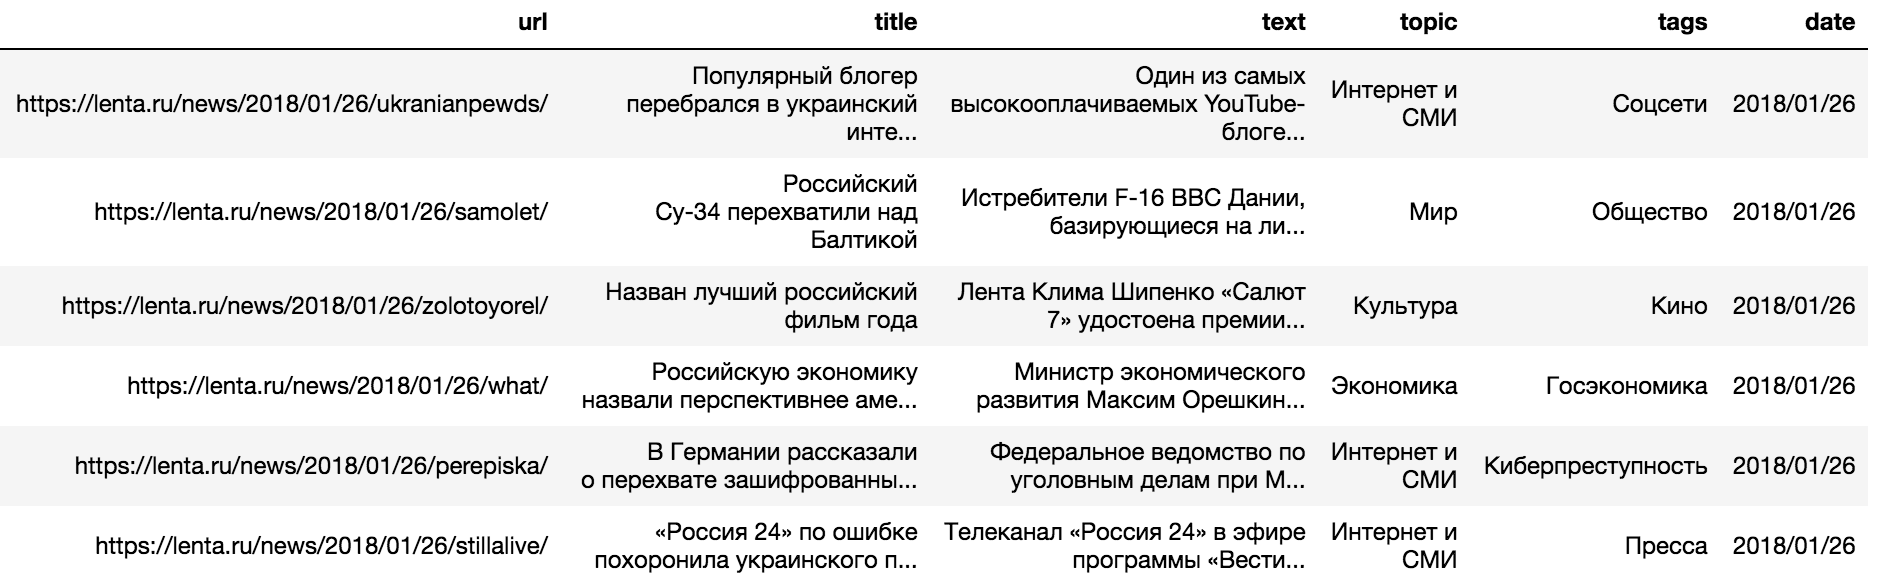
\includegraphics[scale=0.55]{f1.png}\\
\\
\tabЦелевой переменной для классификации могут выступать topic, tags. Заметим, что значений tags больше и они конкретнее, чем значения topic. Пример значений topic: Библиотека, Россия, Мир, Экономика, Спорт, тогда как в tags входит Музыка, Люди, Звери, Игры, Госэкономика, Гаджеты, Наука, Еда, Рынки, Деньги, Летние виды, Интернет и многое другое. Исходя из этого, целевой переменной для первичной модели можно взять tags, исключив topic из модели.\\
\tabИз графика распределения количества новостей с различными темами видно, что лидирует тема "Россия", "Мир". Однако, новости с этими темами могут содержать информацию как о политике, так и о происшествиях, событиях. То есть информация, содержащаяся в topic недостоверна, поэтому её не стоит включать в модели.\\
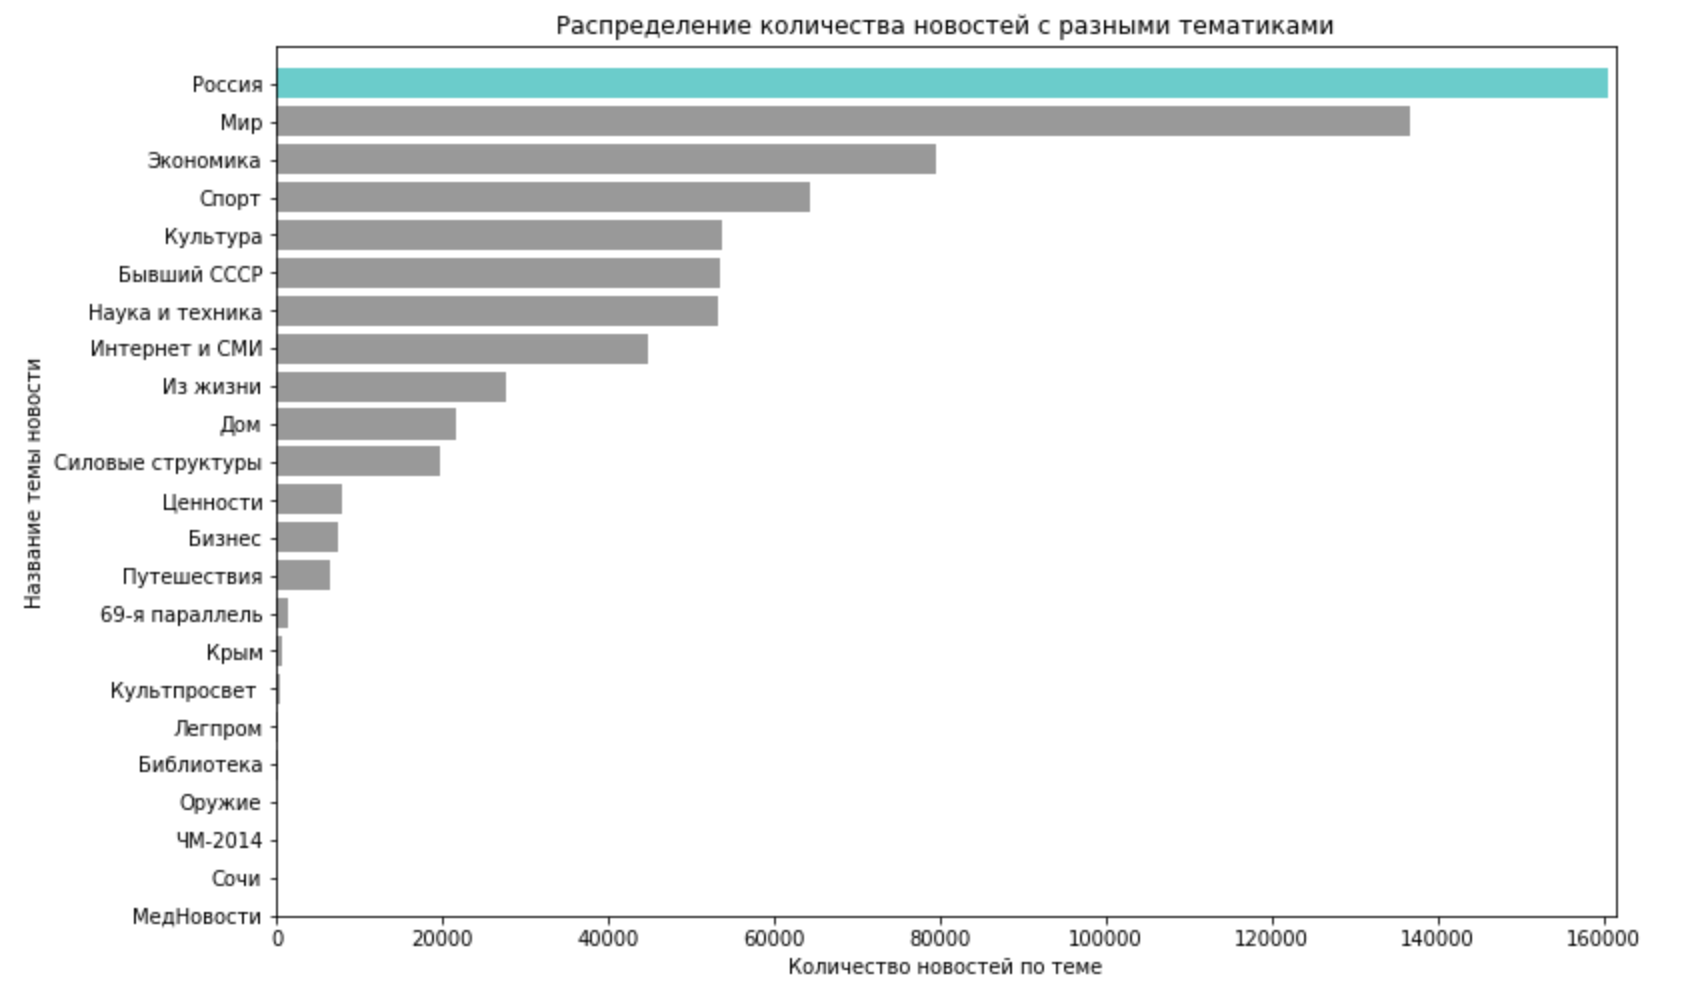
\includegraphics[scale=0.6]{f2.png}\\
\tabИзучив распределение тегов, можно сделать вывод о том, что они подробнее описывают содержание новости. Выделяется тег "Все", которым отмечены новости совершенно разных направленностей, поэтому соответствующие данные были удалены из датасета.\\
\\
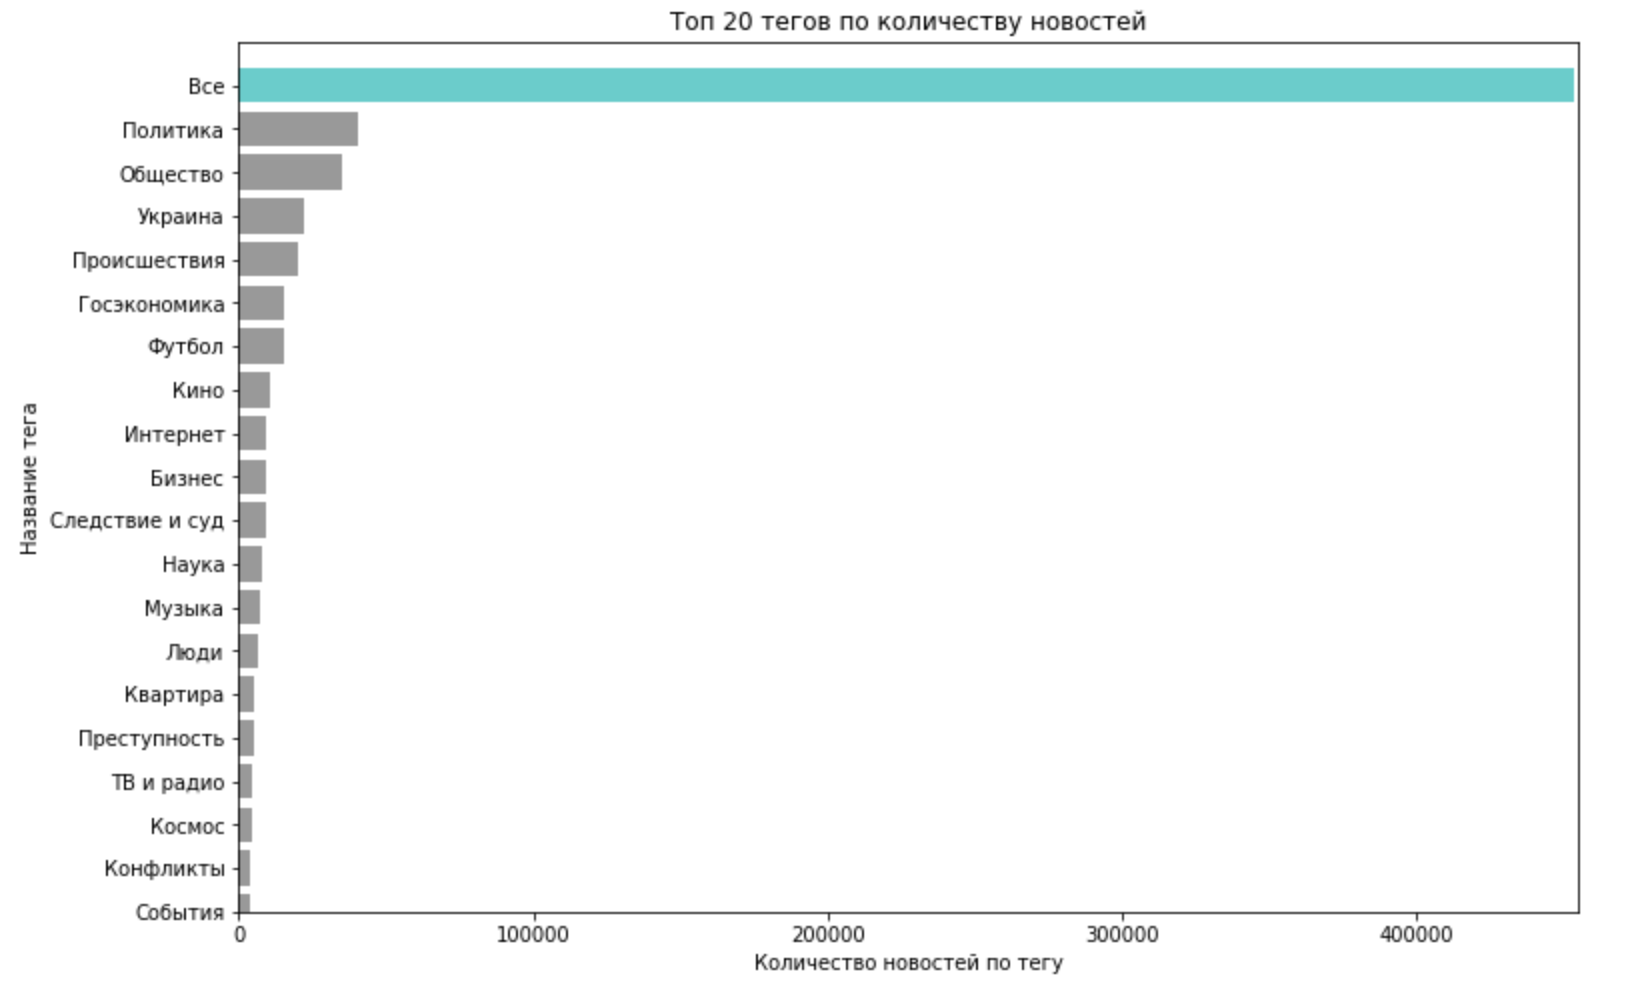
\includegraphics[scale=0.6]{f3.png}\\
%--------------------------------------------------------------------
\subsection{Работа с пропущенными значениями}
\tabПроверим присутствие пропущенных значений в датасете, так как большинство алгоритмов NLP с ними не работают. Пропуски есть в колонках topic, tags, text. Эти колонки являются важными для моделей классификации, поэтому удалим новости, содержащие пропущенные значения.\\\\
\tab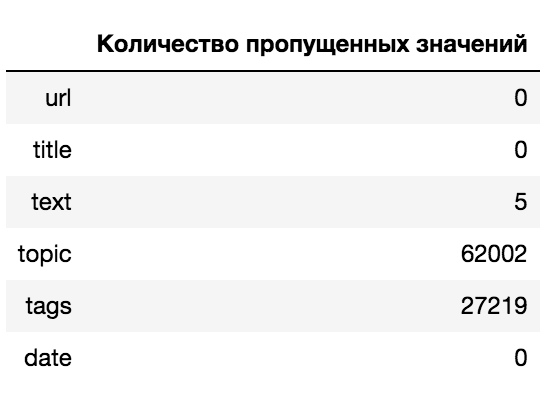
\includegraphics[scale=0.8]{f4.png}\\
\tabТакже удалим колонку url с информацией о ссылке на новость, так как она не несет смысловой нагрузки для дальнейшей работы.\\
%--------------------------------------------------------------------
\subsection{Предварительная обработка данных}
\tabВозьмем данные за 2018 год. Проверим распределение количества новостей по тегам. Из графика видны частотные теги: Политика, Общество, Футбол и мало-частотные: Экология, Наследие, Выборы. распределение получилось с тяжелым хвостом, поэтому для улучшения качества работы модели из данных были исключены новости с тегами, количество которых не превышало 1000. Распределение до и после обработки:\\
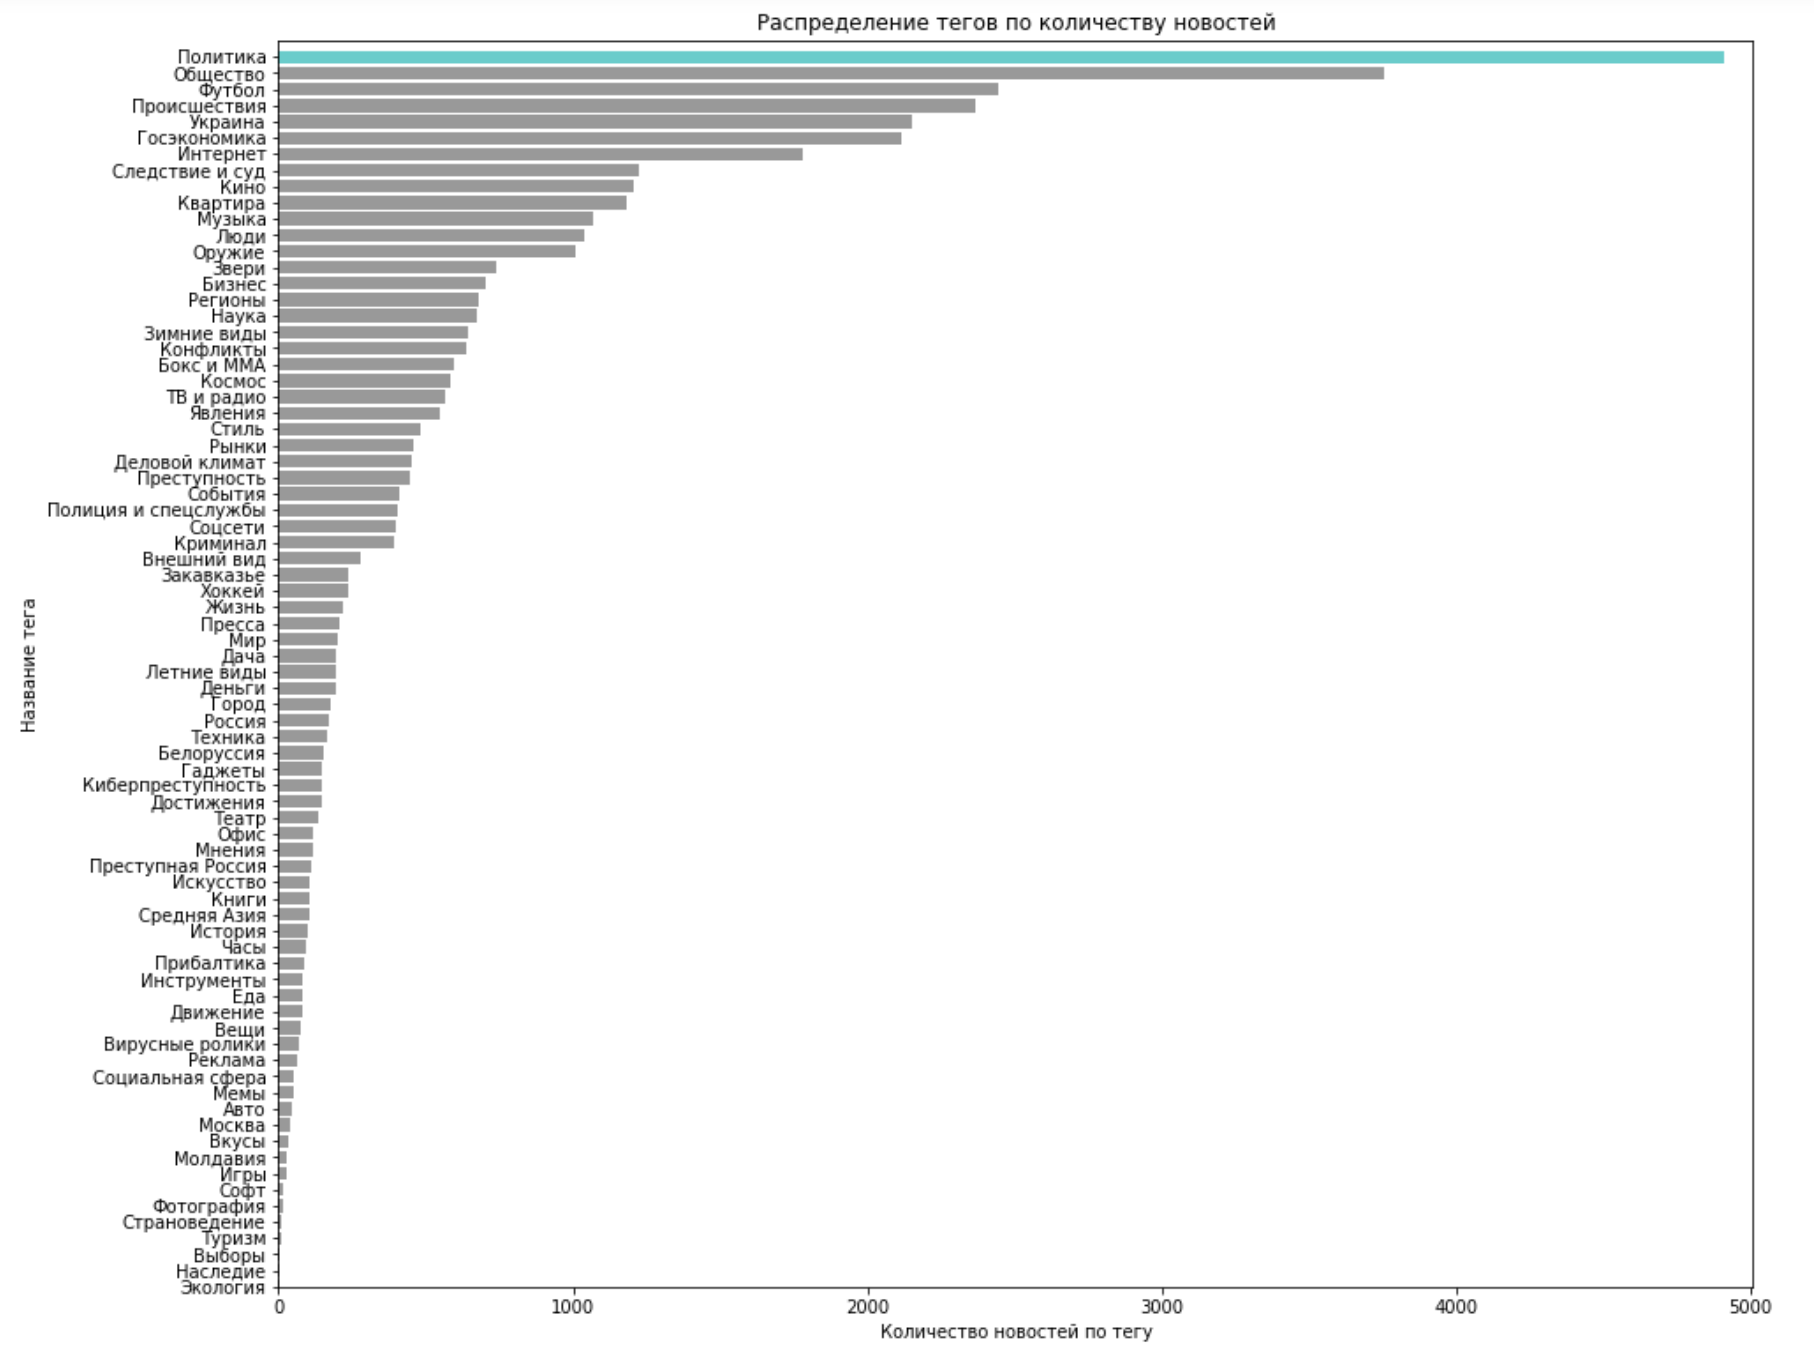
\includegraphics[scale=0.6]{f7.png}\\
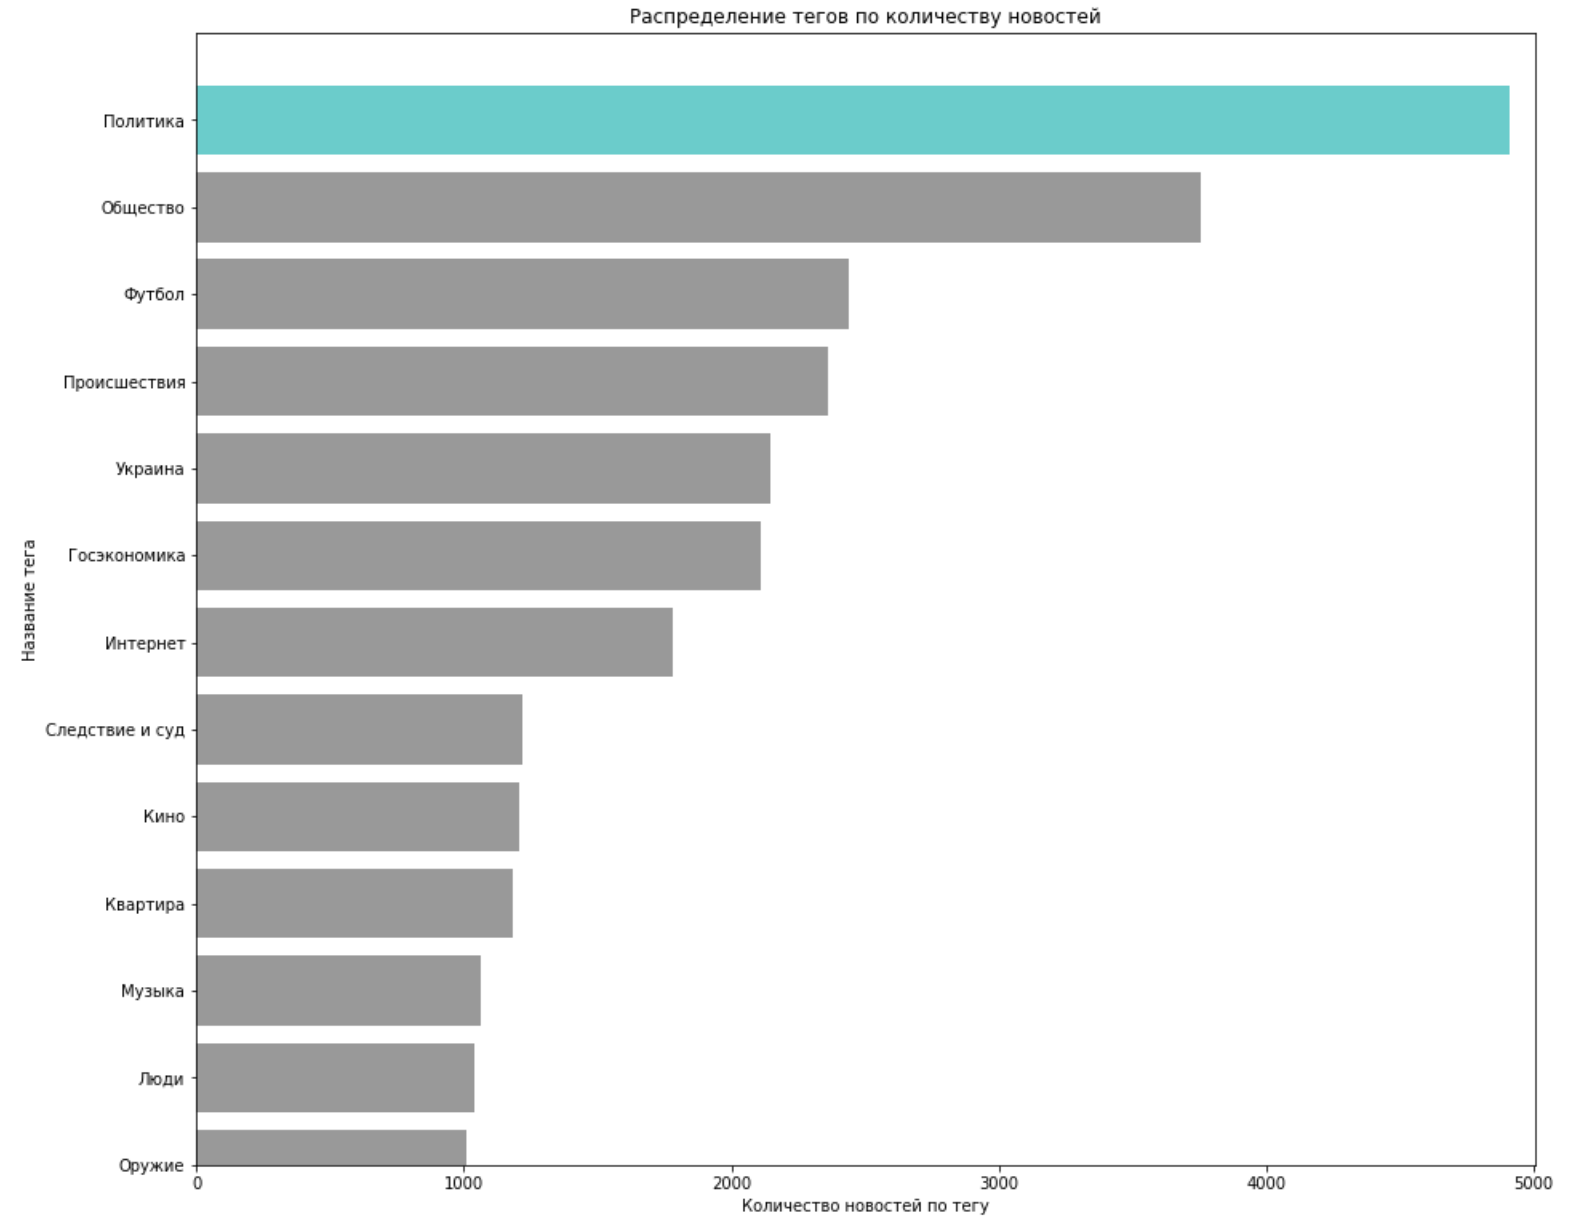
\includegraphics[scale=0.6]{f12.png}\\
\tabРазобьем заголовок новости и текст на токены, то есть на слова. В данной работе рассматривается наиболее гибкий инструмент для токенизации текста – регулярные выражения. Слова были приведены к нижнему регистру. Далее, из текста с помощью регулярного выражения извлекаются все слова, при этом удаляются цифры, знаки пунктуации, иностранные слова и символы. Из полученного массива удаляются стоп-слова. Корпус стоп-слов для русского языка можно получить из библиотеки nltk. Пример таких слов: 'а', 'без', 'более', 'больше', 'будет', 'будто', 'бы', 'был', 'была', 'были', 'было' и так далее. Однако, библиотека содержит информацию о 151 слове и является неполной, поэтому из электронного ресурса был скачан дополненный список, содержащий 421 слово. \\
%--------------------------------------------------------------------
\subsubsection{Лемматизация}
\tabПосле всех вышеперечисленных преобразований с помощью библиотеки pymorphy2 производится лемматизация оставшихся слов. По исходной словоформе и тегам выполняется поиск нормальной формы слова. Для анализа неизвестных слов в Pymorphy2 используются несколько методов, которые применяются последовательно. Изначально от слова отсекается префикс из набора известных префиксов и если остаток слова был найден в словаре, то отсеченный префикс приписывается к результатам разбора. Если этот метод не сработал, то аналогичные действия выполняются для префикса слова длиной от 1 до 5, даже если такой префикс является неизвестным. Затем, в случае неудачи, словоформа разбирается по окончанию. Для этого используется дополнительный автомат всех окончаний, встречающихся в словаре с имеющимися разборами. В процессе построения из автомата удаляются редкие окончания и разборы. Если слово имеет несколько вариантов разбора, то среди всех выбирается наиболее вероятный. Вероятности определяются по следующей формуле:\\
$$P(w|t) = \frac{F_{r}(w,t)+1}{F_{r}(w)+|R(w)|}$$\\
, где $F_{r}(w)$ — количество раз, которое словоформа $w$ встретилась в корпусе\\
\tab$F_{r}(w,t)$ — количество раз, которое эта словоформа встретилась с тегом $t$\\
\tab$|R(w)|$ — число разборов, полученных от анализатора для словоформы $w$\\
\\
\tabПродемонстрируем пример работы функции. Первоначальная новость:\\
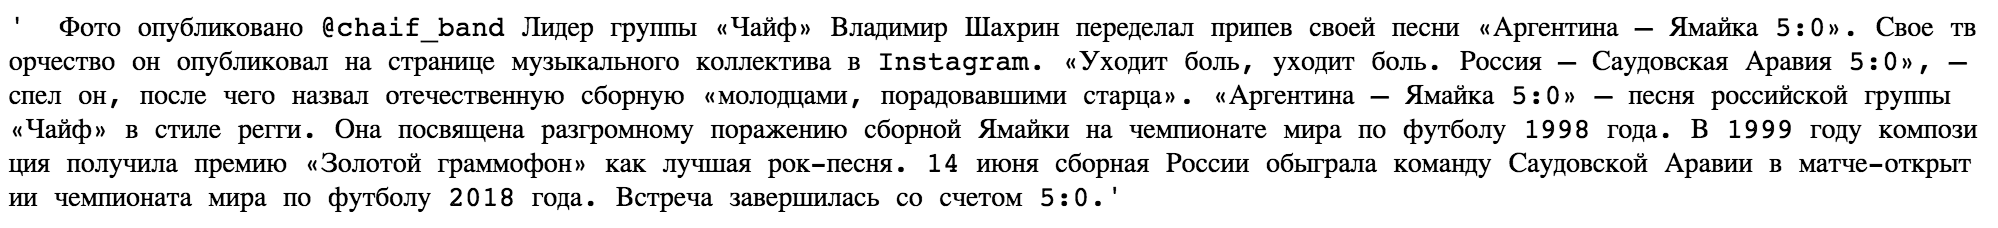
\includegraphics[scale=0.55]{f5.png}\\
\tabПосле обработки:\\
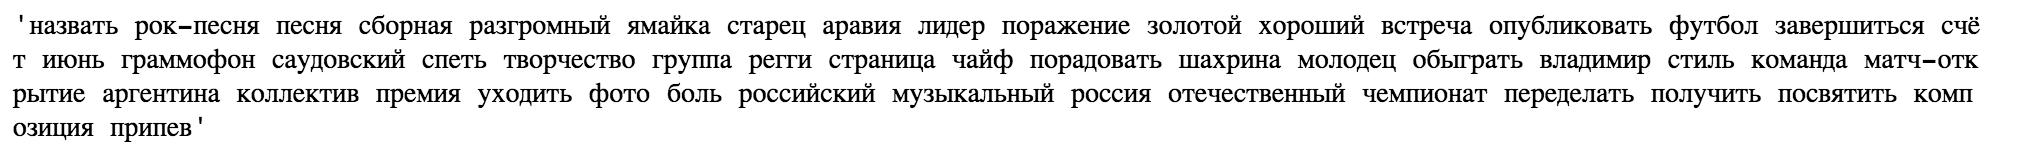
\includegraphics[scale=0.55]{f6.png}\\
\tabИтоговый датасет после лемматизации принял следующий вид:\\
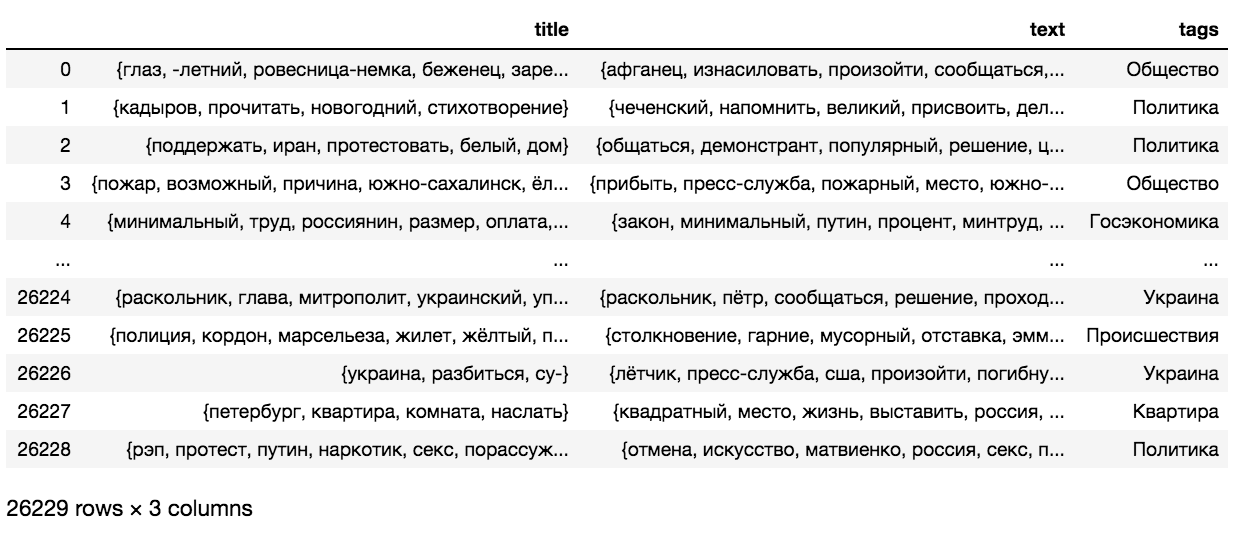
\includegraphics[scale=0.8]{f8.png}\\
%--------------------------------------------------------------------
\subsubsection{Кодирование категориальных данных}
\tabЦелевой переменной для моделей классификации был выбран столбец tags. Можно заметить, что в нём содержатся данные строкового типа, что не подходит для реализации алгоритмов. С помощью функции LabelEncoder из библиотеки sklearn было проведено кодирование признаков, то есть перевод их в числовые значения. Результат преобразования представлен ниже:\\
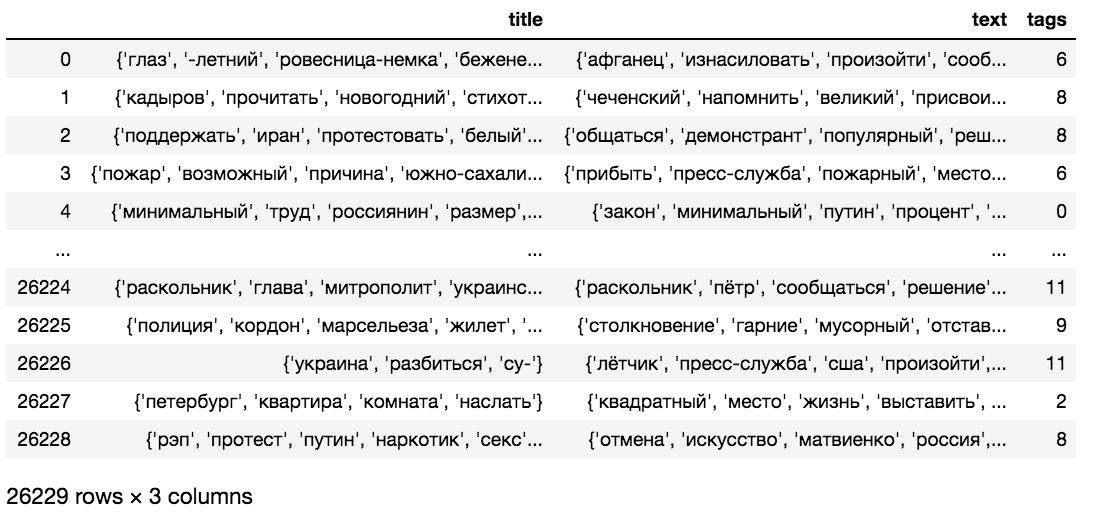
\includegraphics[scale=0.9]{f10.png}\\
%--------------------------------------------------------------------
\subsubsection{TF-IDF преобразование}
\tabДля обучения моделей необходимо получить численные значения из строковых данных. Был использован алгоритм TF-IDF.\\
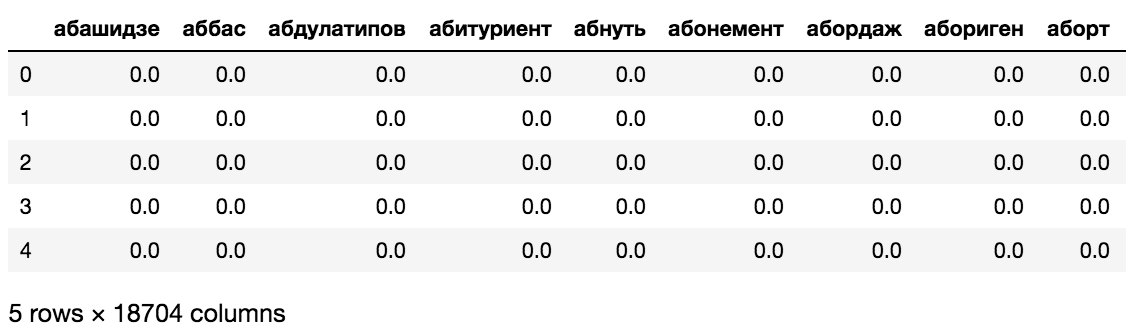
\includegraphics[scale=0.8]{f11.png}\\
\tabСтрочки матрицы соответствуют конкретной новости, индекс которой указан вначале строки. Столбцы соответствуют словам, встреченным в корпусе, состоящем из всех новостей использованного датасета. Значения — коэффициенты TF-IDF. Матрица будет считаться разреженной, то есть матрицей с преимущественно нулевыми элементами. Стоит отметить, что первые три столбца в матрице — вовсе не ошибка, а фамилии политических деятелей, фигурирующих в тексте.
%--------------------------------------------------------------------
\subsection{Разбиение выборки на обучающую и тестовую}
\tabВ любой задаче машинного обучения набор данных разбивается на две выборки: обучающую (train) и тестовую (test). Модель обучают на train выборке, а на test выборке модель проверяют, то есть получают некоторое предсказание. Это необходимо для того, чтобы оценить качество работы алгоритма на уже имеющихся данных и избежать переобучения/недообучения модели. \\
\tabСуществуют несколько способов разбиение данных на выборки. В работе используется разбиение функцией train\_test\_split из библиотеки Sklearn. Функция разбивает данные рандомным способом, что не всегда бывает корректным методом разбиения, но на данном этапе разработки этот метод подходит.\\
%--------------------------------------------------------------------
\subsection{Итоги работы классификаторов}
\begin{center}
\begin{tabular}{||c | c | c||} 
\hline
 Algorithm name & Accuracy & Time \\ [0.5ex] 
 \hline\hline
   GridSearchCV with LinearSVC() & 71.77\% & 13 min. \\  
 \hline
  BaggingClassifier with LinearSVC() & 71.28\% & 4 min. \\  
 \hline
 LinearSVC() & 71.15\% & 2 sec. \\  
 \hline
 SGDClassifier() & 70.8\% & 1 min.\\ 
  \hline
 LogisticRegression() & 69\% & 3 min. \\   
 \hline
 PassiveAggressiveClassifier() &67 \% &  3 min.\\
 \hline
 RandomForestClassifier() & 65\% & 8 min.\\ 
 \hline
 DecisionTreeClassifier() & 57\% & 8 min.\\
 \hline
 MultinomialNB() & 55\% & 1 sec.\\  [1ex] 
 \hline
\end{tabular}
\end{center}\\
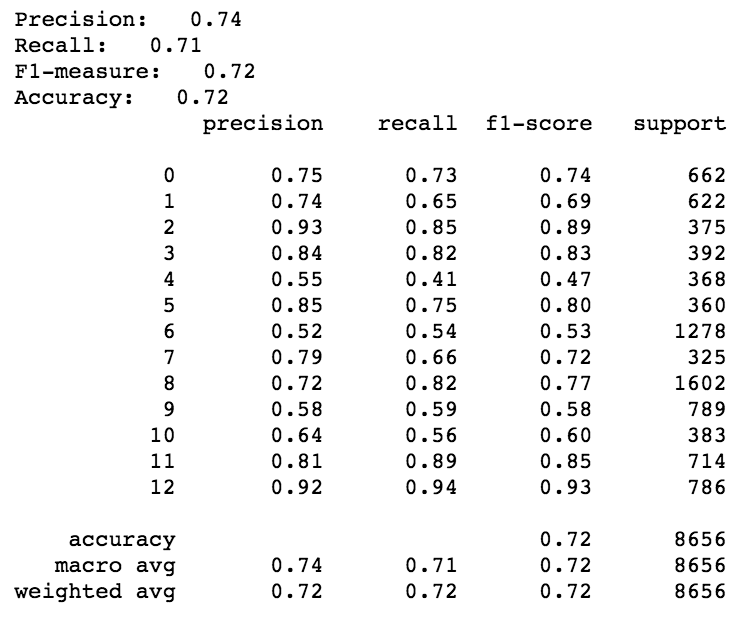
\includegraphics[scale=0.8]{f13.png}\\
\tabНаилучшим образом алгоритм классификации LinearSVC() работает на тегах 'Квартира', 'Кино', 'Музыка', 'Украина', 'Футбол', которым соответствуют категории 2, 3, 5, 11, 12.\\
\tabИз матрицы ошибок видно, что чаще всего классификатор ошибался, относя новости категории Политика, Происшествия к классу Общество. 
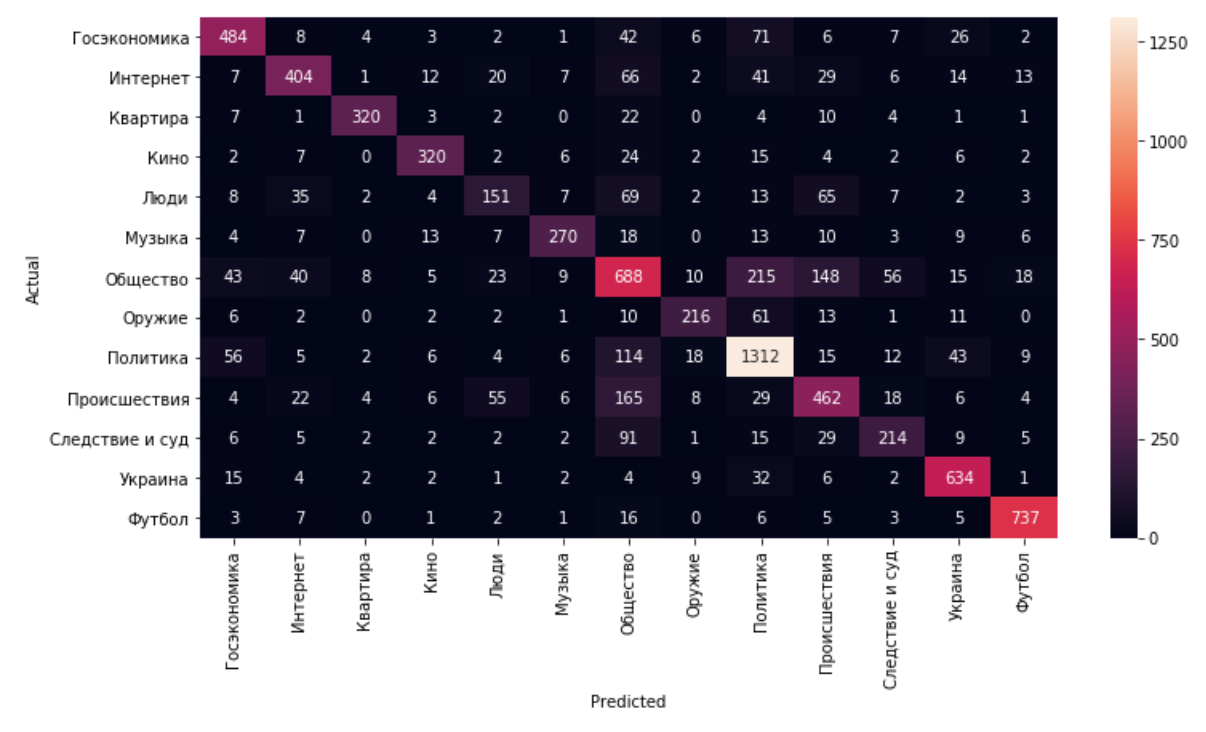
\includegraphics[scale=0.8]{f14.png}\\
%--------------------------------------------------------------------
\newpage
\addcontentsline{toc}{section}{Заключение}
\section*{Заключение}
%--------------------------------------------------------------------
\newpage
\addcontentsline{toc}{section}{Список использованных источников}
\section*{Список использованных источников}
\renewcommand{\refname}{}
\begin{thebibliography}{7}
\bibitem{i1} Applied Text Analysis with Python by Benjamin Bengfort, Rebecca Bilbro, and Tony Ojeda (O’Reilly). ISBN 978­–1­–491­9630-4­-3
\bibitem{i2} Автоматическая обработка текстов на естественном языке и анализ данных : учеб. пособие / Большакова Е.И., Воронцов К.В., Ефремова Н.Э., Клышинский Э.С., Лукашевич Н.В., Сапин А.С. — М.: Изд-во НИУ ВШЭ, 2017. — 269 с. ISBN 978–5–9909752-1-7
\bibitem{i3}МЕТОДЫ И МОДЕЛИ АВТОМАТИЧЕСКОГО ИЗВЛЕЧЕНИЯ КЛЮЧЕВЫХ СЛОВ, С.О. Шереметьева, П.Г. Осминин Вестник ЮУрГУ. Серия «Лингвистика». 2015. Т. 12, No 1. С. 76–81
\bibitem{i4}https://countwordsfree.com/stopwords/russian
\bibitem{i5}Automated News Categorization using Machine Learning methods, U. Suleymanov and S. Rustamov
\bibitem{i6}Applying Machine Learning Algorithms for News Articles Categorization: Using SVM and kNN with TF-IDF Approach
\bibitem{i7}A Comparative Analysis Of News Categorization Using Machine Learning Approaches, Nabamita Deb, Vishesh Jha, Alok K Panjiyar, Roshan Kr Gupta
\bibitem{i8}https://serokell.io/blog/machine-learning-algorithm-classification-overview
\end{thebibliography}
%--------------------------------------------------------------------
\newpage
\addcontentsline{toc}{section}{Приложение}
\section*{Приложение}
\tabИсходный код можно найти по \href{https://github.com/dokapoka/paper_text_classification}{ссылке}.

 \end{document}  